\subsection{齐性空间上的相对不变测度}

再次设 G 是局部紧群，H 是闭子群，\(\beta\) 是 H 上的左 Haar 测度。

引理 6. --- 设 \(\lambda\) 是 G/H 上的测度，\(\chi\) 是 G 到 C* 的连续表示。以下性质等价：

\begin{enumerate}
\def\labelenumi{\alph{enumi})}
\item
  \(\lambda\) 在 G/H 上关于乘子 \(\chi\) 相对不变；
\item
  \(\lambda^{\sharp}\) 在 G 上以左乘子 \(\chi\) 相对不变；
\item
  \(\lambda^{\sharp}\) 具有 \(a\chi \cdot \mu\) 的形式（\(a \in \mathbf{C}\)）。
\end{enumerate}

条件 a) 意味着，对于每个 \(s \in G\)，

\[
\pmb {\gamma} _ {\mathrm{G/H}} (s) \lambda = \chi (s) ^ {- 1} \lambda ;
\]

这等价于 \(\left(\pmb{\gamma}_{\mathrm{G / H}}(s)\lambda\right)^{\sharp} = \chi (s)^{-1}\lambda^{\sharp}\)，即

\[
\gamma_ {G} (s) \lambda^ {\sharp} = \chi (s) ^ {- 1} \lambda^ {\sharp}.
\]

从而 a) 与 b) 等价。b) 与 c) 的等价性由 §1, No.~8, Prop. 10 的 Cor. 1 得出。

定理 3. --- 设 G 是局部紧群，H 是 G 的闭子群，\(\mu\)（分别为 \(\beta\)）是 G（分别为 H）上的左 Haar 测度，\(\chi\) 是 G 到 C* 的连续表示。

\begin{enumerate}
\def\labelenumi{\alph{enumi})}
\item
G/H 上存在关于 G 相对不变且乘子为 \(\chi\) 的非零测度的充要条件是，\(\chi(\xi)=\Delta_{\mathrm{H}}(\xi)/\Delta_{\mathrm{G}}(\xi)\)，对所有 \(\xi\in H\) 成立。
\item
  此时该测度除常数因子外唯一；更精确地说，它与 \((\chi \cdot \mu) / \beta\) 成比例。
\end{enumerate}

G/H 上存在关于 G 相对不变且乘子为 \(\chi\) 的非零测度的充要条件是（引理 6），\(\chi\cdot\mu\) 具有 \(\lambda^{\sharp}\) 的形式，因而（No.~2, Prop. 4）有 \(\boldsymbol{\delta}(\xi)(\chi\cdot\mu)=\Delta_{\mathrm{H}}(\xi)(\chi\cdot\mu)\)，对所有 \(\xi\in H\) 成立。此条件也可写作 \(\chi(\xi)\chi\cdot\Delta_{\mathrm{G}}(\xi)\mu=\Delta_{\mathrm{H}}(\xi)\chi\cdot\mu\)，即

\[
\chi (\xi) = \Delta_ {\mathrm{H}} (\xi) / \Delta_ {\mathrm{G}} (\xi)
\]

对所有 \(\xi \in \mathbf{H}\) 成立。由此得 a)。b) 的断言立即由引理 6 以及映射 \(\lambda \mapsto \lambda^{\sharp}\) 为单射这一事实得出。

\pandocbounded{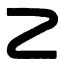
\includegraphics[keepaspectratio]{images/part001_024ad5fd.jpg}}

我们将在 §3（No.~3, Example 4）中看到一些非常简单的例子，在这些例子中，表示 \(\xi \mapsto \Delta_{\mathrm{H}}(\xi) / \Delta_{\mathrm{G}}(\xi)\) 不能延拓为 G 到 \(\mathbf{C}^*\) 的连续表示。因此在这种情形下，G/H 上不存在关于 G 相对不变的非零复测度。

推论 1. --- G/H 上存在关于 G 相对不变的非零正测度的充要条件是，存在一个 \(\mathbf{G}\) 到 \(\mathbf{R}_+^*\) 的连续表示，延拓表示 \(\xi \mapsto \Delta_{\mathrm{H}}(\xi) / \Delta_{\mathrm{G}}(\xi)\)。

注意，当 H 是幺模的，此条件得到满足。

推论 2. --- G/H 上存在关于 G 不变的非零正测度的充要条件是，\(\Delta_{G}\) 与 \(\Delta_{H}\) 在 H 上一致。

推论 3. --- 假设 H 是幺模的，并且 G/H 上存在关于 G 相对不变的非零有界正测度 \(\nu\)。则 \(\nu\) 是不变的，且 G 是幺模的。

  令 \(\chi\) 为 \(\nu\) 的乘子。对于每个 \(s \in G\)，\(\nu\) 与 \(\pmb{\gamma}(s)\nu\) 具有相同的有限总质量（§1, No.~1, 公式 (6)）；由于 \(\pmb{\gamma}(s)\nu = \chi(s)^{-1}\nu\)，有 \(\chi(s) = 1\)。因此 \(\nu\) 不变。由推论 2，\(\Delta_G(s) = 1\)，对所有 \(s \in H\) 成立。令 \(G'\) 为 \(t \in G\) 满足 \(\Delta_G(t) = 1\) 的集合。这是 \(G\) 的包含 \(H\) 的闭正规子群。令 \(\pi\) 为从 \(G/H\) 到 \(G/G'\) 的典范映射。则 \(\pi(\nu)\) 是关于 \(G\) 不变的非零有界正测度。因此，群 \(G/G'\) 的左 Haar 测度有界，从而 \(G/G'\) 是紧的（§1, No.~2, Prop. 2）。所以 \(G\) 在 \(\Delta_G\) 下的像是 \(\mathbf{R}_+^*\) 的紧子群；该子群只能是 \(\{1\}\)，故 \(\Delta_G = 1\) 在 \(G\) 上处处成立。

